\part{Projektdokumentation}

\chapter{Anforderungs- und Problemanalyse}
Aufgabe der Anforderungsanalyse in diesem Projekt war es herauszufinden welches Problem die Kundin mit der zu entwickelnden Software lösen möchte. Dafür wurden Interviews mit dem Kunden durchgeführt und entsprechende Ergebnisse mit Hilfe von Audioaufzeichnung, Mitschriften und Fotografien protokolliert. Zur detaillierten Beschreibung einzelner Abläufe des Systems wurden Kreativtechniken wie das Zeichnen verschiedener Szenarien an einem Whiteboard sowie die manuelle Simulation des Fahrstuhles mit einem aus Pappe gefertigten Modells durchgeführt.
\begin{figure}[hbt]
\hspace*{-1.2cm}
\subcaptionbox{Skizze der Fahrstuhlsimulation am Whiteboard}[0.49\linewidth]
{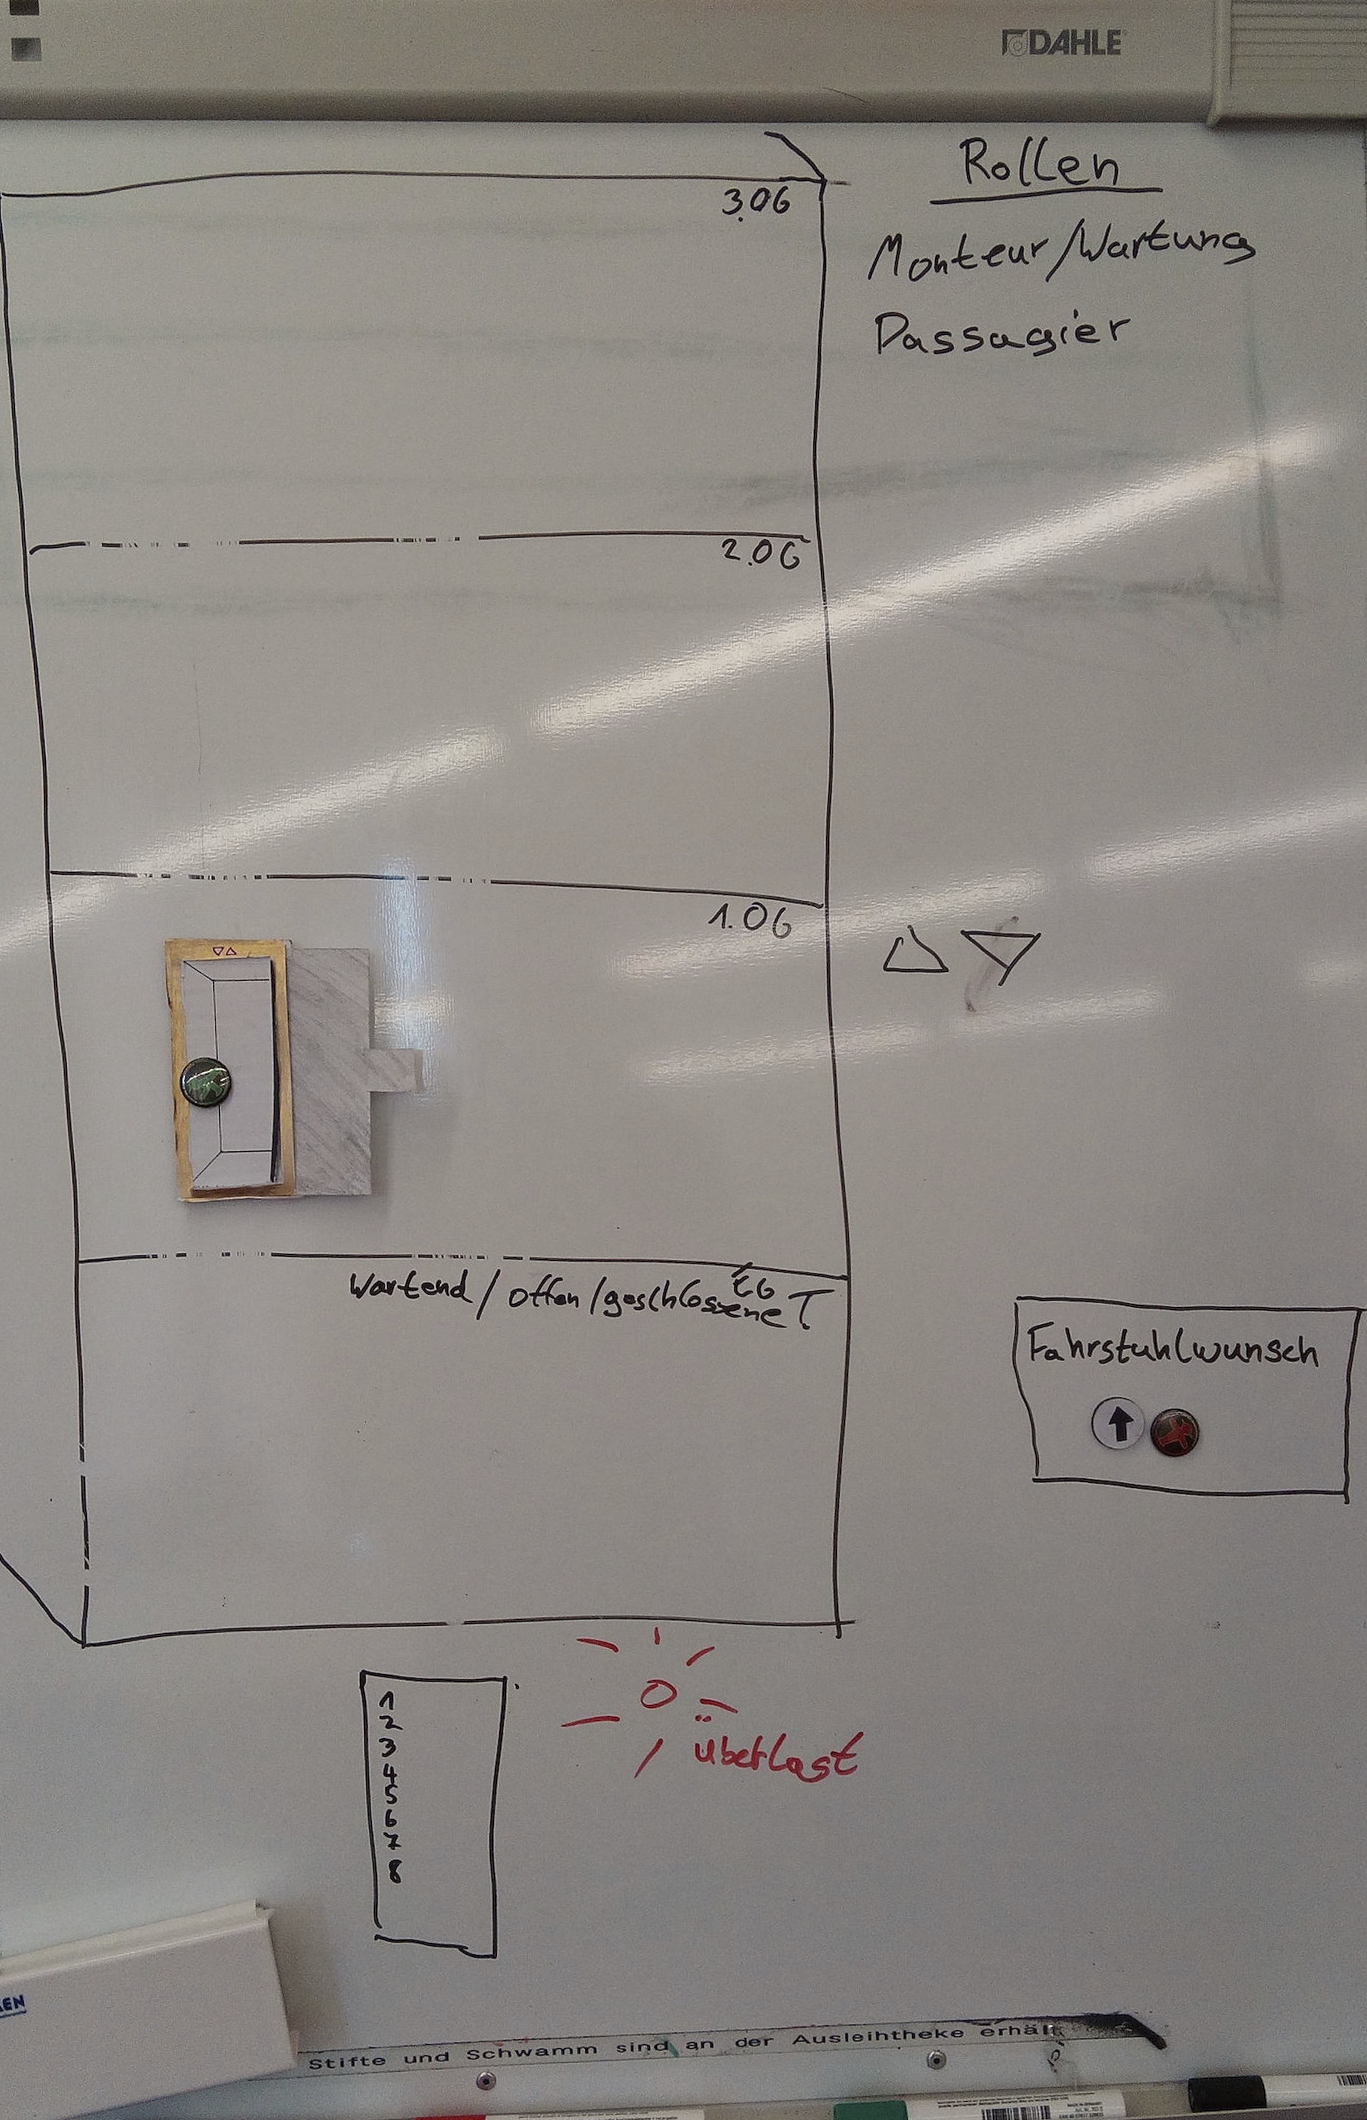
\includegraphics[height=8cm]{images/kundengespraech1.jpg}}
\subcaptionbox{Modell des Fahrstuhles}[0.49\linewidth]
{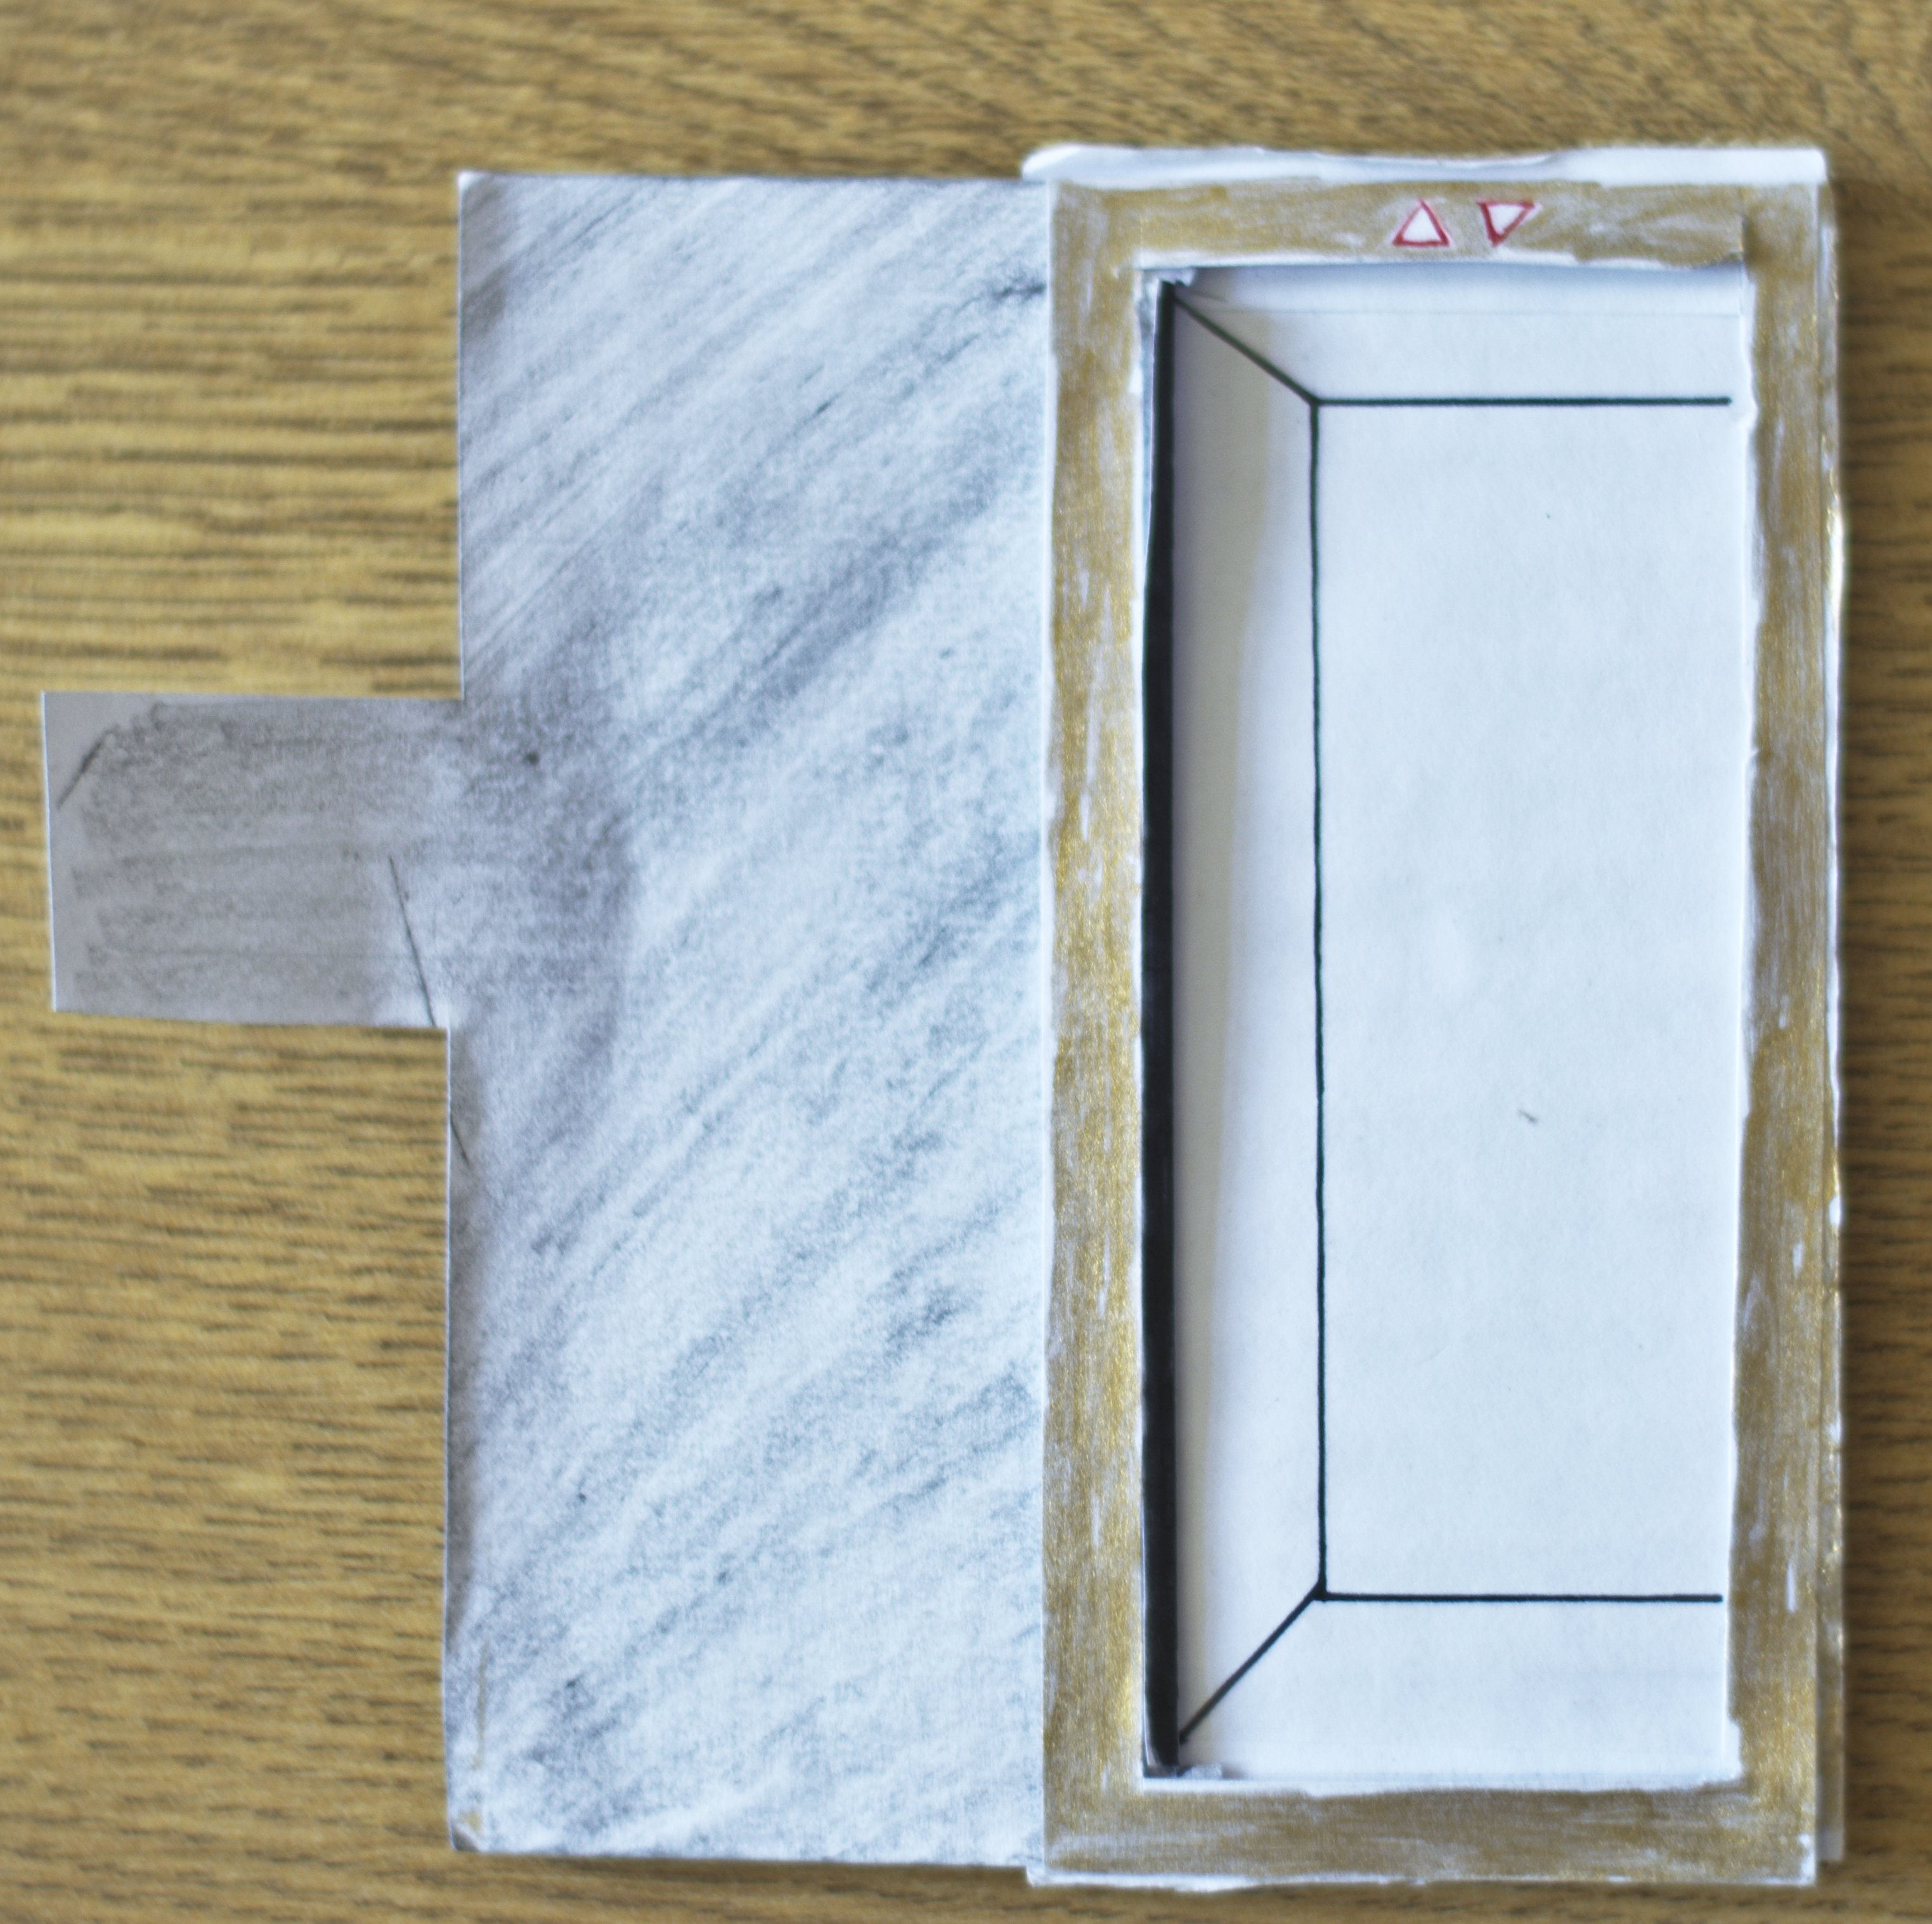
\includegraphics[height=8cm]{images/pappfahrstuhl.jpg}}
\caption{Kreativtechniken zur Anforderungsanalyse}
\end{figure}
Die folgenden grundlegende Fragen waren im Laufe der Analyse zu klären:
\begin{itemize}
	\item Wie viele Fahrstühle sollen verwendet werden können?
	\item Wie soll das Gebäude beschaffen sein?
	\item Welcher Algorithmus soll verwendet werden?
	\item Gibt es Schnittstellen zu anderen Systemen?
\end{itemize}
Weiterhin musste festgelegt werden ob die Priorität des Systems auf der Simulation oder auf einer möglichst realitätsnahen Umsetzung eines Liftes liegt. Im Laufe der Analyse und Modellierung entsprechender Anwendungsfälle wurde ersichtlich, dass das System sich aus zwei Teilsystemen, der \textbf{Fahrstuhlsteuerung} und der \textbf{Fahrstuhlsimulation} zusammensetzt, deren Anforderungen getrennt voneinander beschrieben werden mussten.\\
Eine Besonderheit des Systems ist dabei die Umgebung in der es eingesetzt werden soll, der Lehrbetrieb an einer Hochschule. Daraus ergaben sich spezielle Anforderungen, wie das Anzeigen der Zustandsübergänge, die gesondert betrachtet werden mussten.

\paragraph{}Vor allem aus den letztgenannten Anforderungen formte sich während der Analyse relativ früh unsere Vision einer Anwendung, welche in einer zweigeteilten Sicht Fahrstuhl und Zustandsdiagramm nebeneinander darstellt. Zusätzlich sollten Zustandsübergänge und aktive Zustände durch Animationen kenntlich gemacht werden.

\paragraph*{}Die Resultate der Analysephase, alle Anwendungsfälle und Vereinbarungen mit der Kundin wurden am Ende im Pflichtenheft festgehalten, welches als eigenständiges Dokument am Ende der Phase an die Kundin überreicht wurde. Diese Dokument war im weiteren Verlauf des Projektes ein zentrales Maß bei regelmäßigen Treffen und Evaluationen.



\chapter{Software-Entwurf}
Nach der Festlegung von Anforderungen und der Beschreibung der Funktionalitäten der Fahrstuhlsimulation war der nächste Schritt der Entwurf der internen Struktur. Wir näherten uns dieser Problemstellung von außen und erhöhten bei steigender Tiefe die Granularität. Dies bedeutete zunächst, die geeignetste Rahmen-Technologie festzulegen, welche die Anforderungen unseren Kundin am besten erfüllen konnte.

\section{Technologie}
Die Wahl der verwendeten Technologie fußte prinzipiell auf drei Hauptpunkten, erstens unserer Vision einer optisch ansprechenden Anwendung, welche das Zusammenspiel von System und dessen Zuständen visualisiert. Zweitens einer möglichst umfassenden Kompatibilität zu verschiedenen Plattformen und drittens der verfügbaren Zeit zur Realisierung aller Anforderungen. Wir entschlossen uns zunächst eine Vorauswahl zu treffen. Diese sollte wenn möglich Technologien enthalten, auf deren Gebieten bereits Erfahrungen im Team vorhanden waren. Nach kurzer Diskussion ergaben sich als Möglichkeiten die Nutzung von \textsc{C++}, \textsc{Java} oder \textsc{Web-Technologien} wie \textsc{Javascript}.

\paragraph*{}Nach reiflicher Überlegung und wiederholter Rücksprache mit unserer Kundin erschienen uns \textsc{Web-Technologien} am geeignetsten um alle Anforderungen in der zur Verfügung stehenden Zeit umzusetzen. Die Vorteile dieser Technologien, welche unsere Entscheidung maßgeblich beeinflussten, waren folgende:

\begin{enumerate}
	\item Sie ermöglichten uns größtmögliche Plattform-Kompa\-tibilität, da unser Produkt einerseits als Cross-Plattfom-Anwendung und andererseits als Web-Site veröffentlicht werden können.
	\item Mit den modernen Mitteln des Web-Designs war es uns möglich unsere Vision des Software-System umzusetzen.
\end{enumerate}

Gebündelt und verwendet wurden diese Möglichkeiten durch modere Werkzeuge der Web-Entwicklung wie beispielsweise \textsc{ReactJS}\footnote{\url{http://facebook.github.io/react/}}, \textsc{nodeJS}\footnote{\url{https://nodejs.org}}, \textsc{bower}\footnote{\url{http://bower.io}} oder \textsc{grunt}\footnote{\url{http://gruntjs.com}}. An dieser Stelle verweisen wir auf die entsprechenden Stellen der Entwicklerdokumentation.

\section{Algorithmus}
Bei der Wahl des zu implementierenden Fahrstuhl-Algorithmus lies uns die Kundin freie Hand. Im Kundengespräch wurde auch über die mögliche Erweiterung der Software um mehrere Algorithmen diskutiert. Dies hatte den Charme, dass Studierende damit zusätzlich die Möglichkeit gehabt hätten verschiedene Algorithmen zu vergleichen und zu erfahren wie stark oder weniger stark sich verschiedene Ansätze einer Problemlösung im Hinblick auf Algorithmus und Zustandsdiagramm unterscheiden. Letztlich wurde diese Erweiterung als \textit{mögliche Modifizierung} kategorisiert und ist nicht Teil dieses Projekts geworden.

\paragraph{}Wir entschieden uns im folgenden dazu einen Algorithmus zu verwenden, welcher in Fahrstuhlsystemen mit einem Schacht Anwendung findet, den \textit{Fahrstuhl-Algorithmus mit Sammelsteuerung}\cite{wiki_elev}. Hierbei fährt der Fahrstuhl zunächst in eine Richtung und bedient ausschließlich Fahrtwünsche oder -rufe die in dieser Fahrtrichtung existieren, andere werden gespeichert und nach Umkehr der Fahrtrichtung bedient.

\begin{figure}[h]
	\begin{minipage}{0.47\textwidth}
		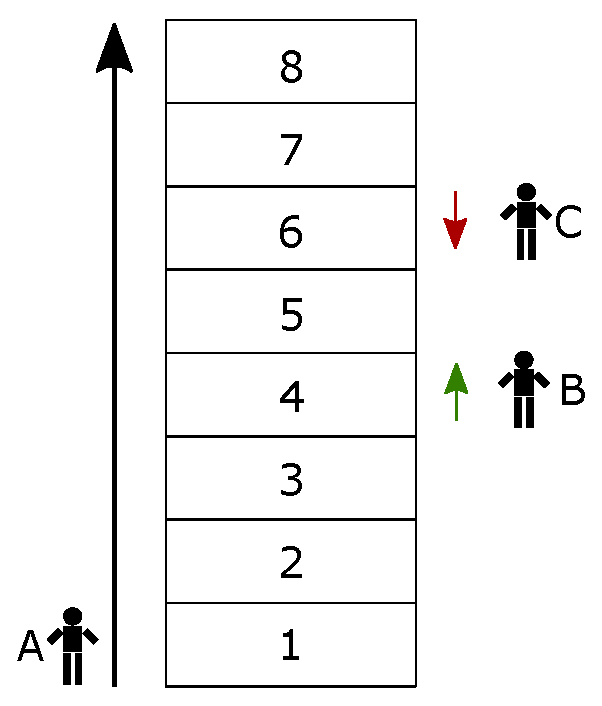
\includegraphics[width=\textwidth]{images/algo_example.eps}
		%\caption{Eine Grafik}
		%\label{Bild}
	\end{minipage}
	% Auffüllen des Zwischenraums
	\hfill
	% minipage mit Grafik
	\begin{minipage}{0.47\textwidth}
		\paragraph{Beispiel}
		Passagier \textbf{A} steigt im Erdgeschoss zu und möchte in den achten Stock fahren. Während sich der Fahrstuhl in Bewegung setzt rufen ihn zwei weitere Personen auf Etage vier und sechs. Person \textbf{B} auf Etage vier ruft \textit{nach oben} und \textbf{C}, jene auf Etage sechs \textit{nach unten}.\\
		Während seiner Fahrt wird der Fahrstuhl nun den Ruf auf Etage vier bedienen, während er an Etage sechs vorbeifährt. Dieser Ruf wird im Anschluss nach Umkehr der Fahrtrichtung bedient.
		% \caption{Der Text}
		% \label{Text}
	\end{minipage}
	\caption{Beispiel zum Fahrstuhl-Algorithmus mit Sammel\-steuerung.}
	\label{algo_exam}
\end{figure}

\paragraph{}Wie man erkennen konnte setzt diese Form der Steuerung zwei Tasten je Etage zur Abgabe von Fahrtstuhlrufen voraus, weshalb diese in der vorliegenden Form implementiert wurden. Für weitere Informationen zu verschiedenen Fahrstuhl-Algorithmen verweisen wir auf folgenden Quellen \cite{wiki_elev} und \cite{wiki_elev_2}.

\newpage
\paragraph{Zustandsdiagramm}Nun galt es den Steuerungsalgorithmus näher zu analysieren, um ihn anschließend mittels \textsc{Javascript} zu implementieren. Dazu wurde über mehrere Gruppentreffen hinweg am Zustandsdiagramm des Systems gearbeitet. Abbildung \ref{ZD} zeigt das Resultat dieser Arbeit.

\begin{figure}[h]
	\hspace*{-2.0cm}
	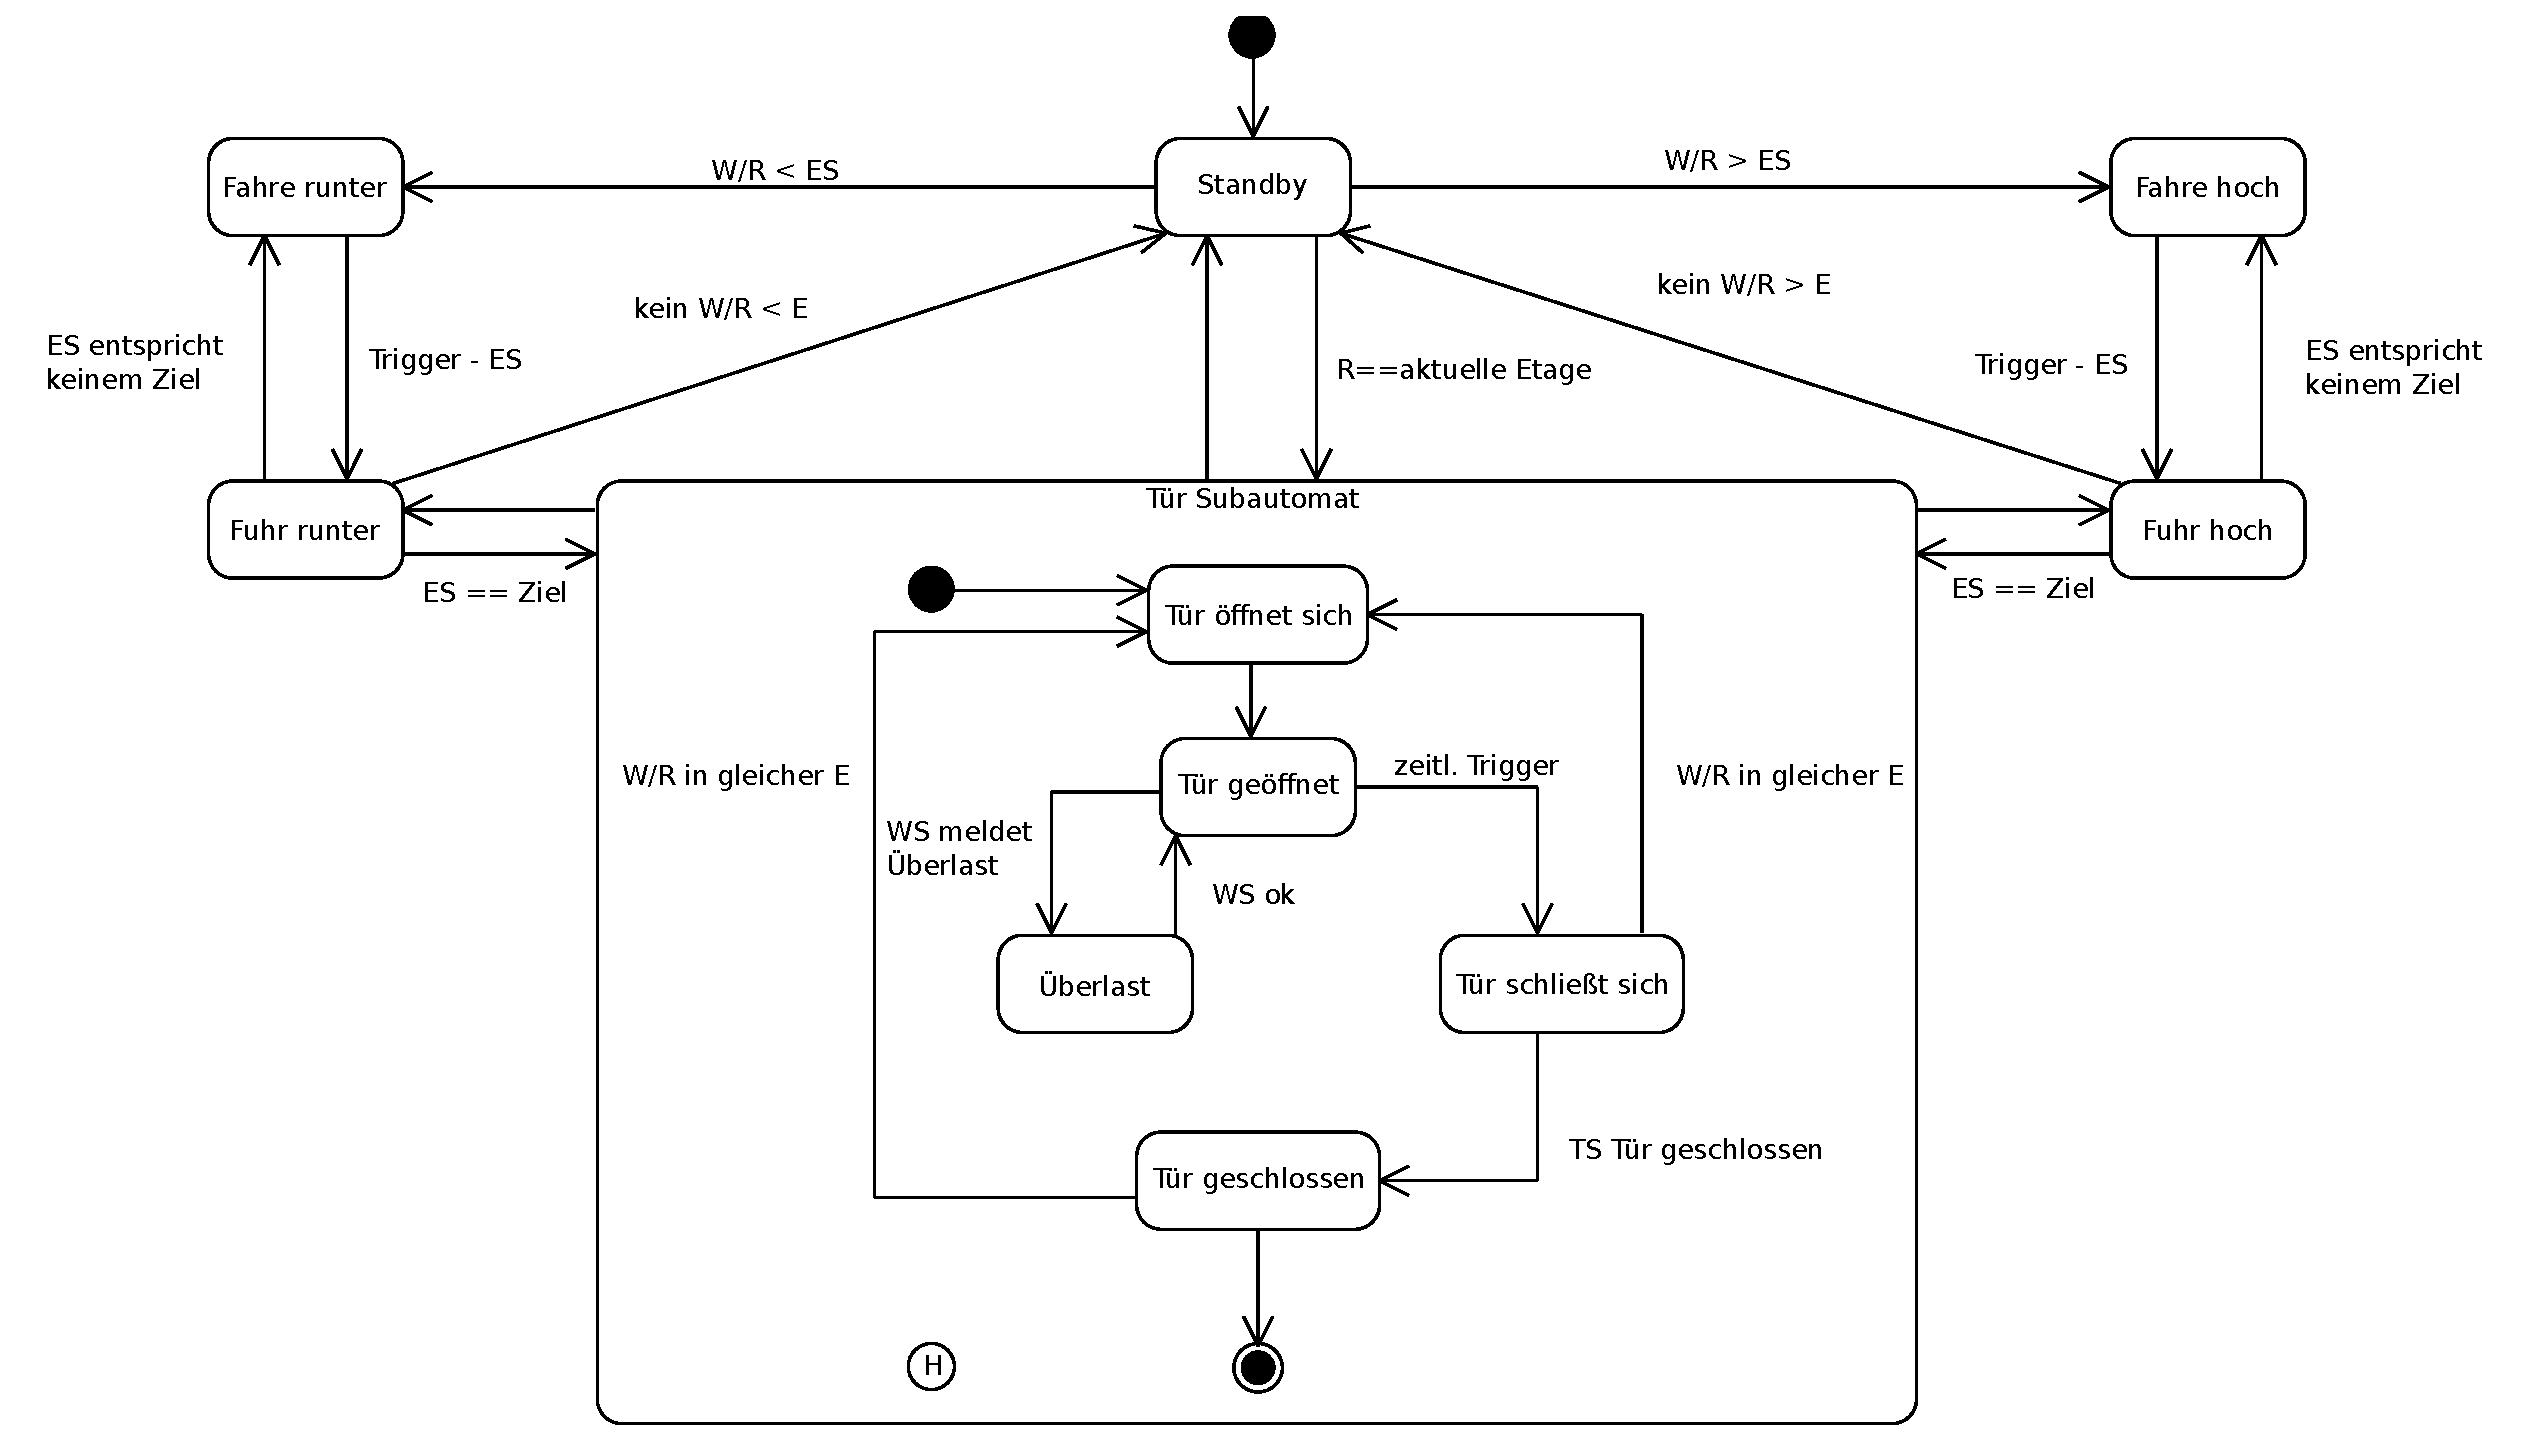
\includegraphics[width=1.3\textwidth]{images/ZDv6.eps}
	\caption{Zustandsdiagramm der Fahrstuhlsteuerung. Die im Diagramm verwendeten Abkürzungen erklären sich folgendermaßen: \textit{W}: Wunsch, \textit{R}: Ruf, \textit{ES}: Etagensensor, \textit{E}: Etage, \textit{WS}: WeightSensor oder Gewichtssensor}
	\label{ZD}
\end{figure}

\paragraph{Fahrt}
Den \textit{Standby}-Zustand nimmt die Steuerung in unserem System sowohl nach dem Start in Etage 1 als auch auf einer beliebigen Etage ein, sofern keine weiteren Wünsche oder Rufe vorhanden sind. Werden nun Rufe abgegeben, entscheidet die Steuerung auf Basis der Summe über und unter ihrer aktuellen Position, in welcher Richtung sie mit der Bearbeitung beginnt.

\paragraph{}Nehmen wir im Folgenden an, dass der Fahrstuhl nach oben fährt. In diesem Fall geht er zunächst in den Zustand \textit{Fahre hoch} über. Die Vorbeifahrt an einem Etagensensor \textit{ES} löst einen Übergang in den Zustand \textit{Fuhr hoch} aus, in welchem ein Mechanismus überprüft, ob die aktuelle Etage einem Wunsch/Ruf entspricht. Ist dies nicht der Fall, wird die Fahrt in der gleichen Richtung fortgesetzt, was dem erneuten Übergang in den Zustand \textit{Fahre hoch} entspricht.\\
Handelt es sich jedoch um eine Zieletage, geht die Steuerung in den \textit{Tür-Subautomat} über. Dieser entspricht einem sogenannten \textit{History-Zustand}\cite{history_Z}, welcher es uns elegant ermöglicht nach dem Verlassen des Subautomaten in einen Zustand gleicher Fahrtrichtung zurückzukehren.

\paragraph{Tür-Subautomat}
Mit dem Eintritt in den Subautomat öffnen sich zunächst die Fahrstuhltür. Im Zustand \textit{Tür geöffnet} können durch Betätigung des entsprechenden Buttons Fahrgäste hinzugefügt oder entfernt werden. Bei einer Anzahl von mehr als 8 Personen löst der Gewichtssensor \textit{ES} einen Übergang ein den Zustand \textit{Überlast} aus, welcher den Fahrstuhl am fahren hindert und nur durch das Entfernen von Passagieren verlassen werden kann.\\
Sollte die Weiterfahrt nicht durch Betätigung der Ruf- oder Wunschtaste der aktuellen Etage verhindert werden, geht der Fahrstuhl nach dem Schließen der Tür in den \textit{Fuhr hoch}-Zustand der letzten Fahrrichtung über.

\paragraph{}Nach der Abarbeitung aller Wünsche und Rufe geht die Steuerung in der aktuellen Etage des Fahrstuhls erneut in den \textit{Standby}-Zustand über.

\section{Benutzerschnittstelle}
Der Prozess, welcher letztlich zur vorliegenden Gestaltung der Benutzerschnittstelle führte, verlief ähnlich dem des Zustandsdiagramms. Über mehrere Treffen hinweg wurden Vorschläge gesammelt, diskutiert und letztlich der Kundin unterbreitet. Ein Zwischenstadium dieses Prozesses zeigt Abbildung \ref{Entwurf_UI}.

\begin{figure}[h!]
	\centering
	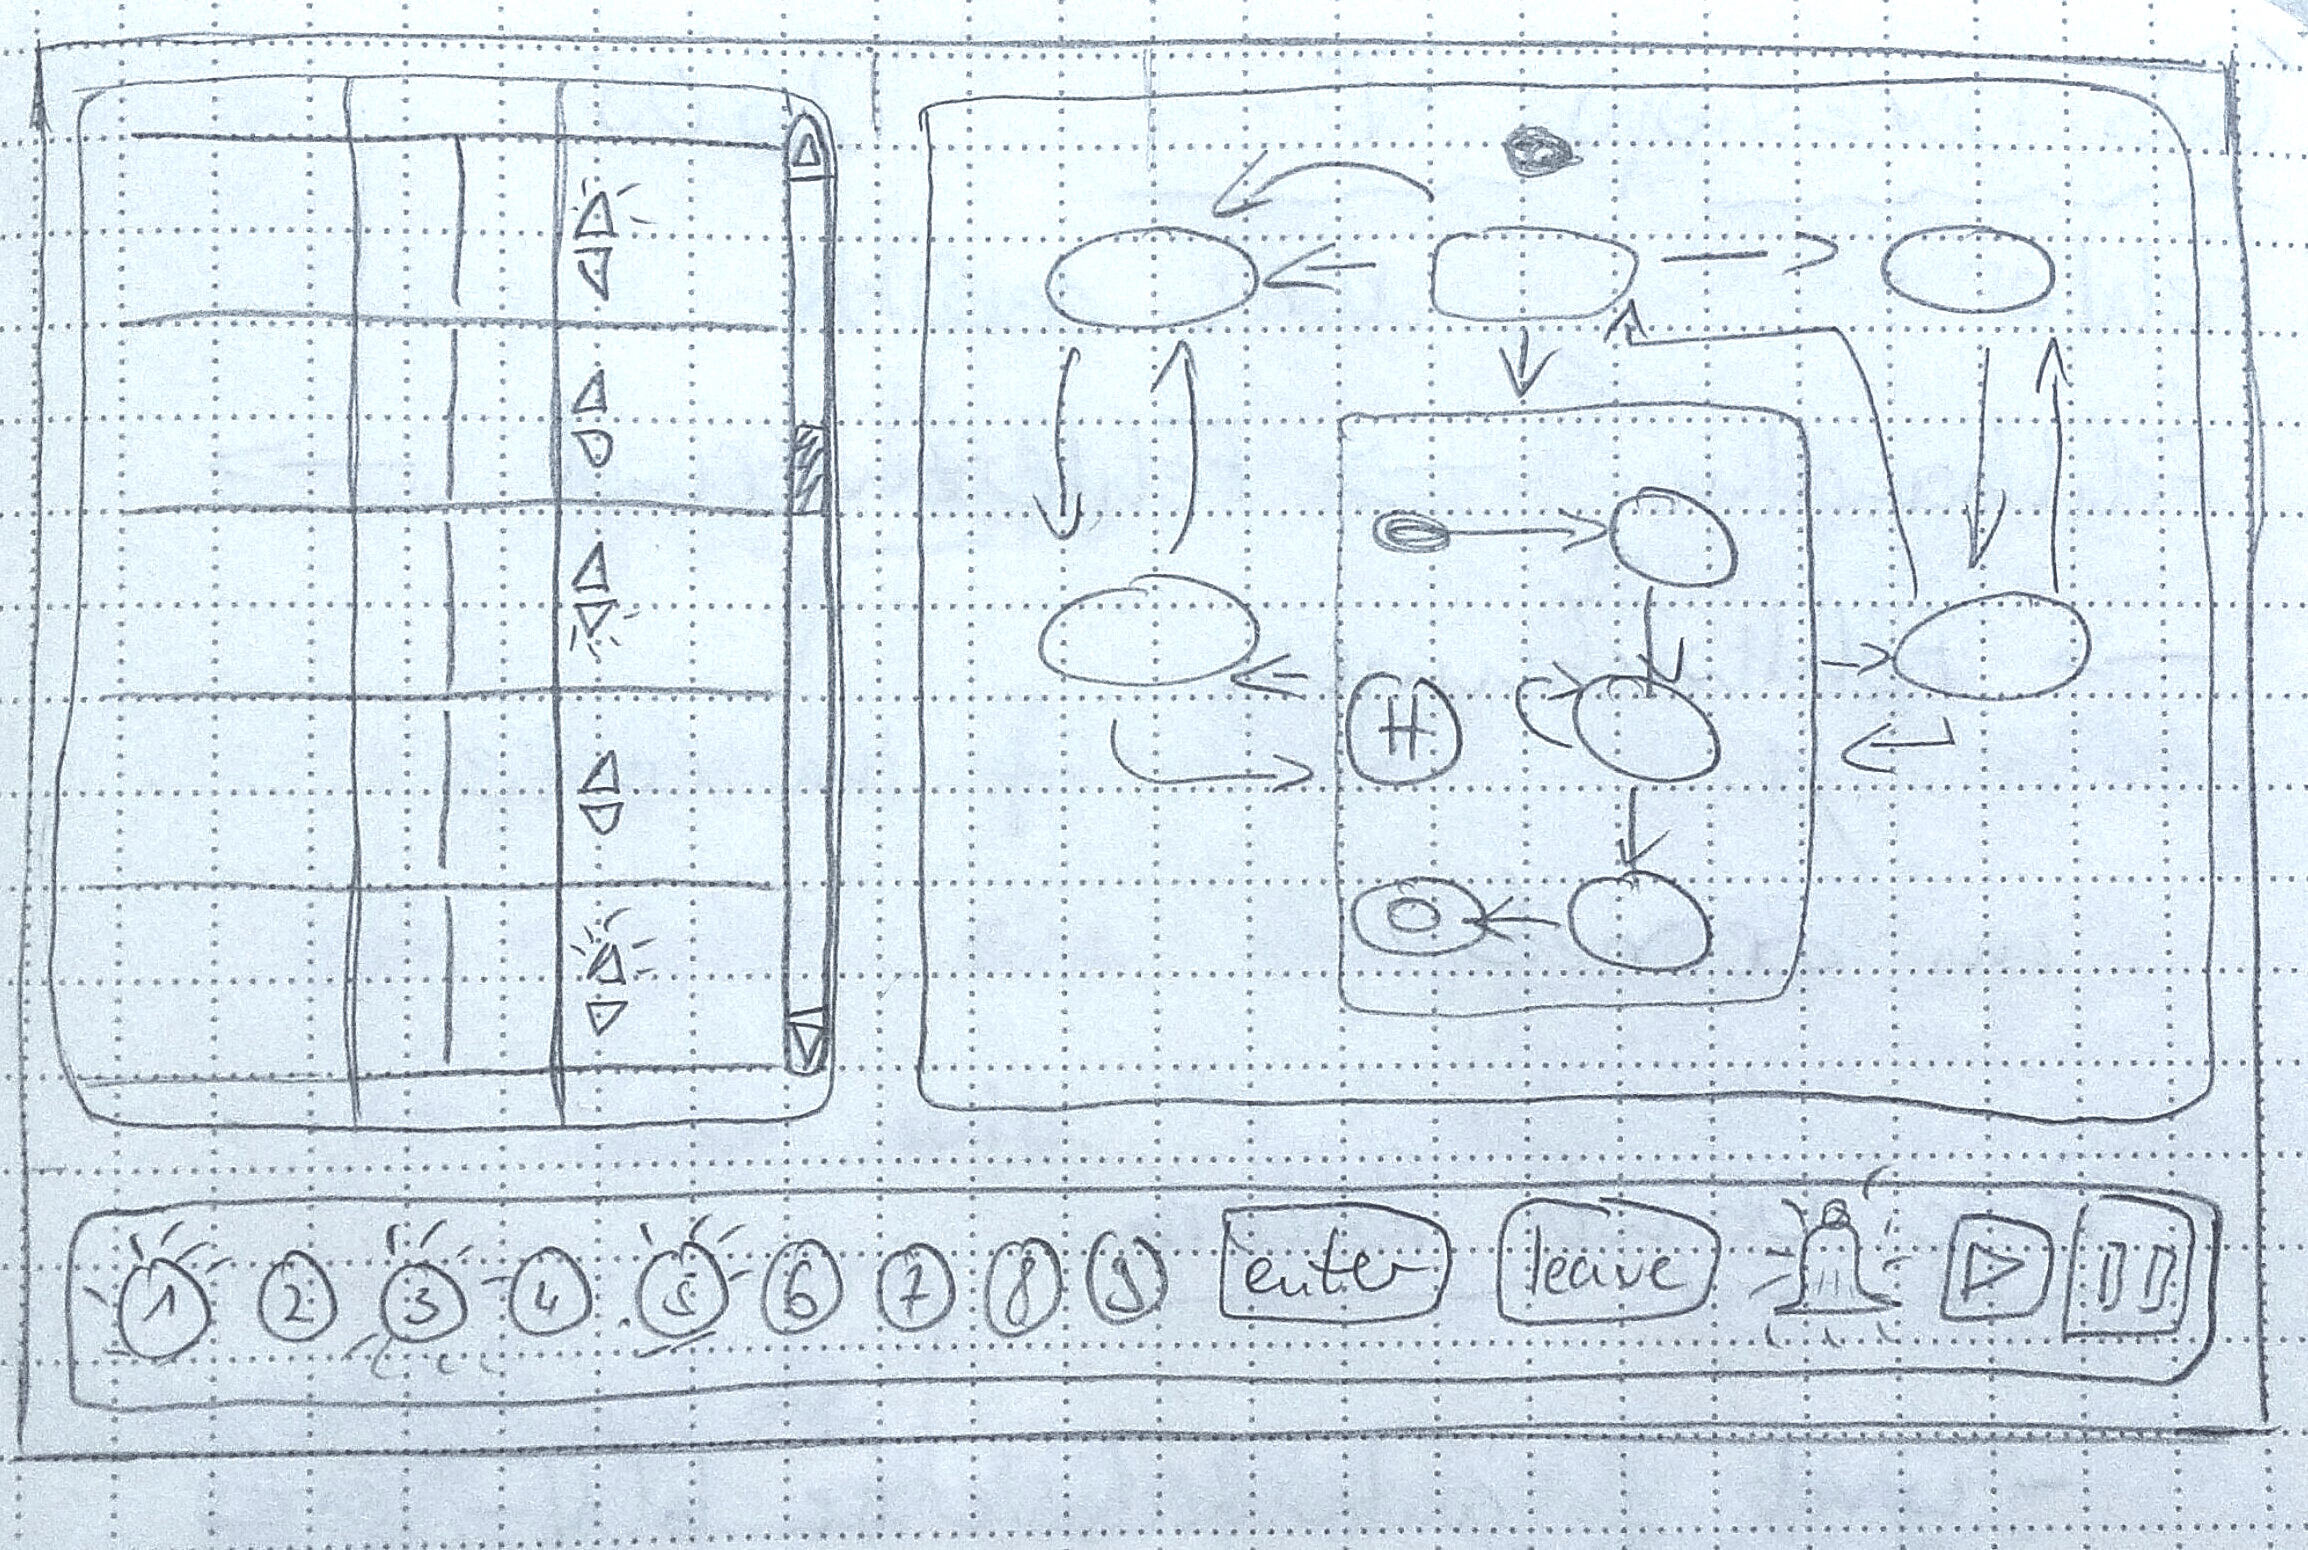
\includegraphics[width=0.8\textwidth]{images/Entwurf_UI}
	\caption{Früher Entwurf der Benutzerschnittstelle. Zu erkennen sind im linken Bereich die Visualisierung des Fahrstuhlschachts sowie die des Zustandsdiagramms im rechten Bereich. Die untere Leiste enthält in diesem Entwurf die Schaltflächen zur Steuerung.}
	\label{Entwurf_UI}
\end{figure}

\hspace*{2cm}
\paragraph{}Im Laufe der Entwicklung wurde die Benutzerschnittstelle stets weiterentwickelt. Nachdem frühe Versionen zunächst nur die Visualisierung des Fahrstuhls enthielten (siehe Abb. \ref{UI_ealry}) zeigt Abbildung \ref{UI_final} die finale Version.

\hspace*{2cm}
\begin{figure}[h!]
	\centering
	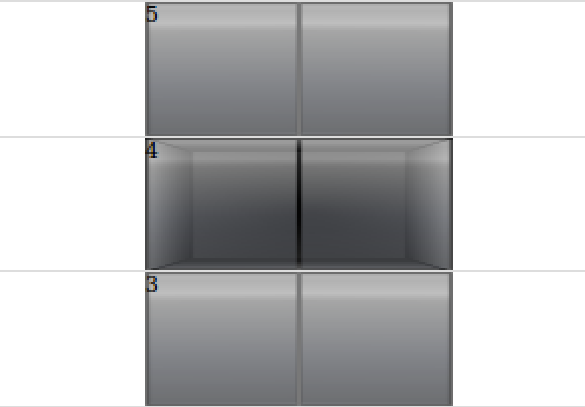
\includegraphics[width=0.5\textwidth]{images/UI_frueh.png}
	\caption{Ausschnitt aus einer frühen Version der Fahrstuhlvisualisierung. Zu erkennen ist der Schacht und die Etagen drei bis fünf. Die Kabine befindet sich gerade in Etage 4.}
	\label{UI_ealry}
\end{figure}

\begin{figure}[h]
	\centering
	\missingfigure{Finale UI}
	\caption{Some caption}
	\label{UI_final}
\end{figure}

\paragraph{}Die Prämissen des Projektes, Studierenden und Lehrenden ein übersichtliches und einfach zu bedienendes Werkzeug an die Hand zu geben, standen auch beim Entwurf der Benutzerschnittstelle immer im Vordergrund.

\section{Komponenten und Design Pattern}
Story? \todo{Wie leiten wir in unserem "from the outside to the inside" Approach am besten auf Architektur und Komponenten um?}

\subsection*{State Design Pattern}
Vorteile, Nachteile, warum haben wir uns dageben entschieden?

\subsection*{Event Emitter}
\subsection*{Observer Pattern}


\chapter{Qualitätssicherung}
\label{QS}
\section{Allgemein}
Der Standard ISO/IEC 25000:2014 welcher als Einleitung zu genormten Methoden der Qualitätssicherung in der Software zu verstehen ist, definiert diese als "`Systems and Software Quality Requirements and Evaluation (SQuaRE)"'\cite[Foreword]{ISO25000}. Festzustellen ist: Der ISO25000 ist für einen Norm relativ jung ist und löst zwei Vorgänger, welche die Themen Softwarequalität bzw. Anforderungsanalyse (ISO/IEC 9126) und Software Evaluierung bzw. Test (ISO/IEC 14598) überwiegend getrennt behandeln ab. Neben der Motivation der Vermeidung von Redundanzen und Inkonsistenzen zwischen den zwei Normen, ist es Meinung des Autors, dass sich hierbei die Erkenntnis der notwendigen Verzahnung der beiden Teilgebiete zeigt. So werden z.B. im \textit{test driven development} idealerweise die Anforderungen direkt zur Software-Evulation benutzt.

\paragraph*{}Aus der Definition
\begin{quote}\label{PD_SQ}
software quality
capability of software product to satisfy stated and implied needs when used unter specified condidtions
\end{quote}\cite[4 Terms and definitions]{ISO25000}
lässt sich somit die umfassende Qualitätssicherung aufteilen auf
\begin{enumerate}
\item Einwirkung auf Anforderungsanalyse
\item Evaluation während und nach der Umsetzung
\end{enumerate}
da sich Softwarequalität nach obiger Definition rein auf die bereits eruierten Anforderungen und Bedingungen stützt, wie Gesamtzufriedenheit des Nutzers allerdings nur dann erreichen lässt, wenn diese Vorbetrachtung bestmöglich durchgeführt wurde.
\section{QS Anforderungsanalyse}
Zu Beginn des Projekts wurde beim der Erstellung des Pflichtenheftes auf vollständige und unmissverständliche Formulierungen geachtet, da Probleme in dieser Phase die größten Auswirkungen auf die Zufriedenheit des Nutzers besitzen.\\
Desweiteren wurde durch erneuten Vergleich der Anforderungen mit Kundenprotokollen und Aufgabenstellung sowie Prüfen auf Inkonsistenzen assistiert.

Als qualitätsunterstüzende Maßnahme wurden die Anforderungen möglichst auf sogenannte Issues, also Stichpunkte und Meilensteine in einem Projektmanager, abgebildet.
\section{QS Umsetzung}
\subsection{Allgemein}
Die Qualitätssicherung während der Umsetzung ließ sich gliedern in:
\begin{itemize}
\item Konvetionen
\item Testregime
\end{itemize}
Desweiteren wurden qualitätssteigernde Maßnahmen durchgeführt, wie das leicht mögliche und oft durchgeführte Review neuer Commits. Siehe dazu \ref{TeamOrg:Werkzeuge}.
\subsection{Konventionen}
Bei der Mitarbeit von mehreren Personen an einem Projekt ergibt sich, durch unterschiedlichen Persönlichkeiten mit verschiedenen Heransgehensweisen und Vorerfahrung, schnell ein Zoo an Stilen und Gewohnheiten. Desweiteren besteht ein gewisser Konsensz, in der Branche, an bestimmen Herangehensweisen und Konvetionen ("`best practice"'). Daraus ergibt sich die Motivation feste Konventionen festzulegen, um entweder Bestehende zu vereinheitlichen oder sie für Jene, welche sie bis dato noch nicht kannten, einzuführen:
%Die Motivation dazu lasse ich hier bewusst herraus, diese möchte ich lieber im Vortrag dazu bennen. Gez. Markus 2015-06-24
\begin{itemize}
\item Allgemeine Konventionen
	\begin{itemize}
	\item Datum- und Zeitangaben sind in ISO 8601 zu notieren, Ausnahmen sind bei nationalen externen Dokumenten möglich
	\item alle Daten sind mit GIT zu Versionieren, temporäre Daten jedoch nicht
	\item alle gefundenen Fehler sind in Issues/Gitlab festzuhalten
	\item Vektorgrafiken sind zu skalieren auf 100x100 px
	\item Textdatein sind in UTF8 zu codieren
	\item Commitmessages und Quelltextkommentare sind in Englisch zu halten
	\end{itemize}
\item Konventionen Quelltext
	\begin{itemize}
	\item camelCase für Bezeichner
	\item keine nachgestellten Leerzeichen\footnote{engl. trailing whitespace}
	\item wenn möglich keine Zeile länger als 80 Zeichen, außer wenn Lesbarkeit sonst herabgesetzt wird
	\item private Member mit einem Unterstrich
	\item Datei endet mit newline (leere Zeile)
	\item Javascript:
		\begin{itemize}
		\item ECMAScript 6
		\item "`use strict"' als erste Zeile eines .js
		\item Tabs statts Space
		\item Einrückungsstil Variante 1TBS \footnote{\url{https://en.wikipedia.org/wiki/Indent_style\#Variant:_1TBS}}
		\end{itemize}
	\end{itemize}
\end{itemize}


\subsection{Test}
Für die automatischen Tests wurde das Testframework Jasmine\footnote{http://jasmine.github.io}
\todo{Traceabillity hinzufügen -> jede Anforderung muss im Quellcode durch einen commit oder ähnlich nachverfolgbar sein}
\subsubsection{manuelle Testfälle}
\begin{testcase}[tc:build]{Manuell}
\tcSubject Projekt-Setup
\tcRemark Testfall um erfolgreichen Build-Prozess garantieren zu können.
\tcConditions
	\begin{enumerate}
	\item Repository mit git geklont
	\item Akutellesten origin/master commit ausgecheckt
	\item Aktuelles Verzeichnis \texttt{se2\_bga} (Projekt-Root)
	\item Alle nicht getrackten Datein gelöscht mit \texttt{git clean -fx}
	\item Alle nicht committeten Datein gelöscht mit \texttt{git reset --hard}
	\end{enumerate}
\tcProceeding
	\begin{enumerate}
	\item Mit NPM verwaltete Abhängigkeiten erzeugen mit \texttt{npm build}
	\item Mit Bower verwaltete Abhängigkeiten erzeugen mit \texttt{bower build}
	\item Build-Jobs mit \texttt{grunt build} ausführen
	\item Wechsel in Verzeichnis \texttt{docs}
	\item Dokumentation setzen mit \texttt{./make\_doc}
	\end{enumerate}
\tcGoal
	\begin{enumerate}
	\item NPM build done without fatal errors
	\item Bower build done without fatal errors
	\item Grunt build done without fatal errors
	\end{enumerate}
\end{testcase}

\begin{testcase}{Manuell}
\tcSubject Fahrstuhlsimulation
\tcRemark Nimmt Bezug auf ELV-001: Die Fahrstuhlsimulation muss den Fahrstuhl nach oben fahren lassen.
\tcConditions
	\begin{enumerate}
	\item Projekt erfolgreich gebaut wie in Test \ref{tc:build} getestet
	\item Im Projekt-Wurzel-Verzeichnis
	\end{enumerate}
\tcProceeding Drücken des Fahrtwunschknopfes "`nach oben"' in einer Etage über dem Ausgangszustand des Fahrstuhls.

\tcGoal Fahrstuhl fährt in gewählte Etage und öffnet Tür.

\tcError Schreiben eines Bugreports via Issue in Gitlab.
\end{testcase}

\subsubsection{automatisierte Testfälle}

\chapter{Team-Organisation}
\section{Gruppenarbeit}
Im Rahmen der vorliegenden Belegarbeit fanden sich Kommilitonen mit verschiedensten Hintergründen in unserem Team zusammen. Unsere Mitglieder waren Diplomstudenten der allgemeinen Informatik aus den Semestern vier und sechs, ein Bachelorstudent im gleichen Studiengang und ein Student der Wirtschaftsinformatik. Unterschiedliche Stundenpläne und Lebenswirklichkeiten machten es zu einer organisatorischen Herausforderungen \glqq \textit{alle unter einen Hut zu bringen}\grqq.

Um unser Team zu organisieren und eine reibungslose Zusammenarbeit zu gewährleisten verwendeten wir verschiedene Strategien und Werkzeuge und legten einige Regeln fest. Beispiele zu letztgenannten wurden im vorherigen Kapitel Qualitätssicherung ab Seite \pageref{QS} beschrieben.

\paragraph{Strategien} Die Zusammenarbeit unseres Teams war von Beginn an \textit{Team-}\textit{betont} und \textit{demokratisch}. Es war uns wichtig Entscheidungen innerhalb der Gruppe zu treffen und jedem Mitglied die Möglichkeit zu geben sowohl an der Entscheidungsfindung teilzuhaben als auch getroffene Entscheidungen zu jedem Zeitpunkt nachvollziehen zu können. Dies setzte ein hohes Maß an Kommunikation voraus, was bis zum Ende einer der Eckpfeiler unseres Teams war.

\paragraph{}Bei der Ausgestaltung der Arbeit verfolgten wir den Ansatz der \textit{simultanen Zusammenarbeit}. Unsere Mitglieder arbeiteten teilweise gemeinsam, zeitweise allein an verschiedenen Problemlösungen und die Koordination dieser Arbeit sowie die Diskussion der Teilergebnisse fand während den zahlreichen Meetings statt.

\paragraph{Meetings}Diese Besprechungen folgten immer einer festen Struktur. Vor dem Stattfindet wurde gemeinsam über die Agenda beraten. Dabei hatte jedes Mitglied die Möglichkeit eigene Punkte aufnehmen zu lassen. Diese Agenda wurde während der Besprechung als Leitfaden betrachtet und alle Diskussionsergebnisse wurden entsprechend ihrer Agendapunkte in einem Protokoll festgehalten. War es bis zum Ende des Termins nicht möglich alle Punkte abzuarbeiten, wurden jene automatisch zur Agenda des nächsten Termins hinzugefügt. Die Protokolle aller Besprechungen wurden für die Team-Mitglieder zu jedem Zeitpunkt abrufbar veröffentlicht.  

\paragraph{}Neben dieser geplanten und statischen Form der Kommunikation wurden im Team ebenfalls verschiedene Werkzeuge benutzt, um in bestimmten Situation direkt miteinander in Kontakt zu treten und zeitkritische Probleme gemeinsam zu lösen.

\section{Kick-Off}

\paragraph{Rollen}
\paragraph{Themen- und Werkzeuge}
\paragraph{Milestones}
\section{Verwendete Werkzeuge}\label{TeamOrg:Werkzeuge}
\paragraph{doodle}
\paragraph{gitlab}
\paragraph{slack}
\section{Resümee}

\bibliographystyle{plaindin}
\bibliography{projektdokumentation}
